\documentclass[a4paper,11pt]{article}
\usepackage{cmap}
\usepackage[cp1251]{inputenc}
\usepackage[english, ukrainian, russian]{babel}
\usepackage[left=2cm,right=1.5cm,top=1cm,bottom=1cm]{geometry}
\usepackage{amssymb}
\usepackage{graphicx}

\begin{document}

\pagenumbering{gobble}


\begin{large}

\begin{center}
\section*{Application of generative functions to the problems of maximum chess arrangements of n figures.}
\end{center}

\medskip

\begin{center}
\textbf{Abstract}
\end{center}

A generating function is a formal structure that is closely related to a numerical sequence, but allows us to manipulate the sequence as a single entity, with the goal of understanding it better. Roughly speaking, generating functions transform problems about sequences into problems about
functions. In this article, we will approach a range of problems, involving placing $n$ chess pieces on an $n\times n$ chessboard so that no two pieces attack each other, using the generating functions approach.

\medskip
\medskip

\hrule height 1pt
\vskip 3pt \hrule

\medskip
\medskip


\section*{Generating functions.}

Given sequence $\{a_{n}\}\in \mathbb{R}$ the generative function for it is defined as: $f(x)=\sum\limits_{n=0}^{\infty}a_{n}x^{n}.$ Generative functions provide a great way to operate over sequences, solve recurrent series, understand different enumeration problems etc.

Lets take a look at a simple example of a famous Euler's problem, and how it can be solved using generating functions.

\textbf{Example 1.1.} Which weights can be weighted using given weights $1$, $2$, $2^{2}$,..., $2^{n}$, ... and in how many ways?

Consider the function $f(x) = (1+x)(1+x^{2})(1+x^{4})...=\prod\limits_{n=0}^{\infty}(1+x^{2^{n}}) = 1+a_{1}x+a_{2}x^{2}+... .$ Here, the $a_{n}$ is exactly the amount of different ways one can add numbers $1,2,2^{2},2^{3},...,2^{k},...$ in order to get $n$. Now we can calculate these $a_{n}$, by first calculating the function $f(x)$. For that, lets multiply it by $(1-x)$: $$(1-x)f(x) = (1-x)\prod\limits_{n=0}^{\infty}(1+x^{2^{n}}) = (1-x^{2})\prod\limits_{n=1}^{\infty}(1+x^{2^{n}}) = (1-x^{4})\prod\limits_{n=2}^{\infty}(1+x^{2^{n}}) = ... = 1$$ By dividing by $(1-x)$: $$f(x) = \frac{1}{1-x} = \sum\limits_{n=0}^{\infty}x^{n}$$ So we have, that $a_{n}=1$ for every $n\in \mathbb{N}\cup\{0\}$. That implies, that there is always exactly one way to weight the $n$ using weights $2^{k}$, $k\in \mathbb{N}\cup\{0\}$.


Generative functions can be used to solve the recurrent series. Take, for example, famous Fibonacci sequence:

\textbf{Example 1.2.}
 $a_{0}=1$, $a_{1}=1$, $a_{n} = a_{n-1}+a_{n-2}$. For it we can write generative function $$f(x) = \sum\limits_{n=0}^{\infty}a_{n}x^{n} =a_{0} + a_{1}x + \sum\limits_{n=2}^{\infty}(a_{n-1} + a_{n-2})x^{n} = $$ $$= a_{0} + a_{1}x + \sum\limits_{n=2}^{\infty}a_{n-1}x^{n} + \sum\limits_{n=2}^{\infty}a_{n-2}x^{n} = 1 + x + \sum\limits_{n=0}^{\infty}a_{n}x^{n+1} - x + \sum\limits_{n=0}^{\infty}a_{n}x^{n+2} = $$ $$= 1 + x\sum\limits_{n=0}^{\infty}a_{n}x^{n} + x^{2}\sum\limits_{n=0}^{\infty}a_{n}x^{n} = 1 + xf(x) + x^{2}f(x).$$ So, we got the following equality: $f(x) = 1 + xf(x) + x^{2}f(x)$. From this, we get the generating function for Fibonacci sequence: $$f(x) = \frac{1}{1 - x - x^{2}}.$$ Now, we can write partial fraction expansion for this function: $$f(x)=\frac{1}{\sqrt{5}}(\frac{1}{1-\frac{1}{2}(1+\sqrt{5})x}-\frac{1}{1-\frac{1}{2}(1-\sqrt{5})x})$$


\section*{Some results for certain types of functions.}

Let's consider the Stirling numbers of the second kind: $s_{n+1}^{k}=k\cdot s_{n}^{k}+s_{n}^{k-1}$, $s_{0}^{0}=1$. For them we can take a look at the family of sequences $a_{n}^{(k)} = s_{n}^{k}$. If we first consider generating function for the sequence $a_{n}^{(1)}=s_{n}^{1}=1$, we get $f_{1}(x)=\sum\limits_{n=0}^{\infty}a_{n}^{(1)}x^{n}=\frac{1}{1-x}$. For the sequence $a_{n}^{(2)}=s_{n}^{2}=s_{n-1}^{2}+1$ we can calculate the generating function as $$f_{2}(x)=1 + \sum\limits_{n=1}^{\infty}a_{n}^{(2)}x^{n}=1 + 2\sum\limits_{n=1}^{\infty}a_{n-1}^{(2)}x^{n}+\sum\limits_{n=1}^{\infty}x^{n}.$$ 
Therefore: $$\sum\limits_{n=1}^{\infty}a_{n}^{(2)}x^{n}-2x \sum\limits_{n=0}^{\infty}a_{n}^{(2)}x^{n} = \sum\limits_{n=1}^{\infty}x^{n} = \frac{1}{1-x}-1.$$ From that we get:
$$f_{2}(x)(1-2x)=\frac{1}{1-x}$$ 
and: $$f_{2}(x) = \frac{1}{(1-x)(1-2x)}$$

Similarly we can get, that the generating functions for sequences $a_{n}^{(k)}$ are $$f_{k}(x)=\frac{1}{(1-x)...(1-kx)}$$


\section*{n queens problem and some approaches.}

The $n$ queens problem is the problem of placing $n$ chess queens on an $n\times n$ chessboard so that no two queens attack each other. Solutions exist for all natural numbers $n$ with the exception of $n = 2$ and $n = 3$. Although the exact number of solutions is only known for $n = 27$, the asymptotic growth rate of the number of solutions is approximately $(0.143 n)^{n}$.

Although the n-queens problem is often commonly used as a benchmark for algorithms that solve combinatorial optimization problems; it has found several real-world applications, including practical task scheduling and assignment, computer resource management, and VLSI testing. [1]

Counting the number of solutions for the n queen problem is not easy. Since no known exact mathematical formula was found, just approximation, the solution�s number became too large to enumerate one by one except for small n.

Interestingly, there is no guarantee to increase the number of solutions as n increases. For instance, the number of solutions for the six-Queen chessboard is less than that for the five-Queen. The $27 \times 27$ board is the highest-order board that has been wholly enumerated in approximately one year for more information see project Q27 on the web.

\section*{Partial solution for some figures.}

Lets consider the following figure: partial bishop~--- the figure, that will only be attacking on one line. We will denote the amount of different ways we can place $k$ such figures on a board $n\times n$ by $b_{n}^{k}$.

\begin{center}
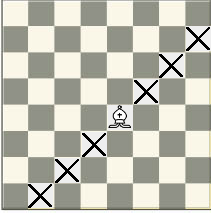
\includegraphics[scale=1]{figure.png}
\end{center}

In case of board $1\times 1$, we get the amount of possible allocations of one such bishop is $1$; so $b_{1}^{1} = 1$ and $b_{1}^{0} = 1$.

Let's assume, that we have the amount of possible allocations of $k$ figures for the board $(n-1)\times (n-1)$. The board $n\times n$ will contain board $(n-1)\times (n-1)$ as it's part (consider lower part to the left, see pic.). If we place $(k-i)$ figures in the part $(n-1)\times (n-1)$, in that case in the remaining $2n-1$ squares we place the rest $i$ figures. But the remaining $2n-1$ slice has only $2n-1-(k-i)$ squares available (as the rest $(k-i)$ squares are under the attack from the already placed $(k-i)$ bishops). That implies the total amount of placements for the remaining slice as $C_{2n-1-(k-i)}^{i}$ (where $C_{n}^{k}=\frac{n!}{(n-k)!k!}$~--- amount of combinations from $n$ to $k$). From that we get, that there are in total $b_{n-1}^{k-i} \cdot C_{2n-1-(k-i)}^{i}$ ways to place $k-i$ figures on $(n-1)\times (n-1)$ part of the board and $i$ figures on the rest of the board.

\begin{center}
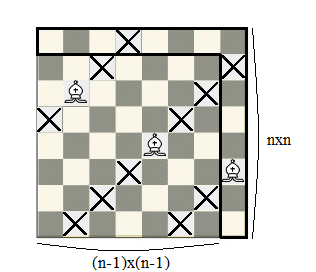
\includegraphics[scale=1]{n_board.png}
\end{center}

By adding all these products for $i=0,1,...,k$ we get the total amount of placements of $k$ figures on the board $n\times n$: $b_{n}^{k}=\sum\limits_{i=0}^{k} b_{n-1}^{k-i} \cdot C_{2n-1-(k-i)}^{i}$.

This way, we have proven the following theorem:

\textbf{Theorem 1.} The amount of possible arrangements of $k$ partial bishops on the board $n\times n$ is given by the following recursive formula: $$b_{n}^{k}=\sum\limits_{i=0}^{k} b_{n-1}^{k-i} \cdot C_{2n-1-(k-i)}^{i} (1)$$

Lets calculate $b_{n}^{k}$ for the case of $k=2$.

\textbf{Theorem 2.} The amount of arrangements of two partial bishops on board $n\times n$ is: $$b_{n}^{(2)} = 1 - 10(n+1)+\frac{29}{2}(n+2)(n+1) + \frac{16}{3}(n+3)(n+2)(n+1) + \frac{1}{2} (n+4)(n+3)(n+2)(n+1).$$

\textit{Proof.} By the recursive formula $(1)$ we have:  $b_{n}^{(2)}=b_{n-1}^{(2)} + b_{n}^{(1)}(2n-2) + \frac{1}{2}b_{n}^{(0)}(2n-1)(2n-2)$. Considering, that $b_{n-1}^{(0)}=1$ and $b_{n-1}^{(1)}=(n-1)^{2}$ (there are always 1 way to place 0 figures on any board and $n^{2}$ ways to place $1$ figure on the board $n\times n$) we get $b_{n}^{(2)}=b_{n-1}^{(2)} + 2n^{3} - 4n^{2} + 3n -1$.

Lets find the generating function for this recursive sequence, and after that, we will be able to find the solution to this sequence. First, we will write down the generative function:
$$f(x) = \sum\limits_{n=1}^{\infty}b_{n}^{(2)}x^{n} = \sum\limits_{n=1}^{\infty}(b_{n-1}^{(2)} + 2n^{3} - 4n^{2} + 3n -1)x^{n} =$$ $$= \sum\limits_{n=1}^{\infty}b_{n-1}^{(2)}x^{n} + \sum\limits_{n=1}^{\infty}2n^{3}x^{n} - \sum\limits_{n=1}^{\infty}4n^{2}x^{n} + \sum\limits_{n=1}^{\infty}3nx^{n} - \sum\limits_{n=1}^{\infty}x^{n}.$$

Therefore, after taking all sums to the left side, we get: $$\sum\limits_{n=1}^{\infty}b_{n}^{(2)}x^{n} - \sum\limits_{n=1}^{\infty}b_{n-1}^{(2)}x^{n} - 2\sum\limits_{n=1}^{\infty}n^{3}x^{n} + 4\sum\limits_{n=1}^{\infty}n^{2}x^{n} - 3\sum\limits_{n=1}^{\infty}nx^{n} + \sum\limits_{n=1}^{\infty}x^{n} = 0 (2)$$

In order to get the value of the generating function, we first have to find the generating functions for sequences $$\sum\limits_{n=1}^{\infty}n^{\alpha}x^{n}.$$ First, we already know, that $$\sum\limits_{n=0}^{\infty}x^{n} = \frac{1}{1-x}$$ (and thus, $\sum\limits_{n=1}^{\infty}x^{n} = \frac{1}{1-x}-1$). Then, $$\sum\limits_{n=1}^{\infty}nx^{n} = x \sum\limits_{n=1}^{\infty}nx^{n-1} = x \sum\limits_{n=1}^{\infty}(x^{n})' = x(\frac{1}{1-x}-1)' = \frac{x}{(1-x)^{2}}.$$ Similarly, we get $$\sum\limits_{n=1}^{\infty}n^{2}x^{n} = x \sum\limits_{n=1}^{\infty}n^{2}x^{n-1} = x \sum\limits_{n=1}^{\infty}n(x^{n})' = x(\frac{x}{(1-x)^{2}})' = \frac{x^{2}+x}{(1-x)^{3}}$$ and $$\sum\limits_{n=1}^{\infty}n^{3}x^{n} = x \sum\limits_{n=1}^{\infty}n^{3}x^{n-1} = x \sum\limits_{n=1}^{\infty}n^{2}(x^{n})' = x(\frac{x^{2}+x}{(1-x)^{3}})' = \frac{x(x^{2}+4x+1)}{(1-x)^{4}}.$$

Now we can use these generating functions (and the fact, that $f(x) = \sum\limits_{n=1}^{\infty}b_{n}^{(2)}x^{n}$) in order to calculate (2): $$f(x)-xf(x) -2\frac{x(x^{2}+4x+1)}{(1-x)^{4}} +4\frac{x^{2}+x}{(1-x)^{3}} -3\frac{x}{(1-x)^{2}} +\frac{1}{1-x} - 1=0.$$ From that result we get that: $$f(x) = \frac{x^{4}+6x^{3}+5x^{2}}{(1-x)^{5}}.$$ Using partial fraction expansion, we get $$f(x) = \frac{1}{1-x}-\frac{10}{(1-x)^{2}}+\frac{29}{(1-x)^{3}}-\frac{32}{(1-x)^{4}}+\frac{12}{(1-x)^{5}}.$$
This way of writing down the generating function is very useful, as we can now, similarly to fibonacci sequence, write down the solution to $b_{n}^{(2)}$. For that, we consider the following: $$\frac{1}{1-x} = \sum\limits_{n=0}^{\infty}x^{n},$$ $$\frac{1}{(1-x)^{2}} = (\frac{1}{1-x})'= (\sum\limits_{n=0}^{\infty}x^{n})' = \sum\limits_{n=0}^{\infty}(x^{n})' = \sum\limits_{n=0}^{\infty}(n+1)x^{n},$$ $$\frac{1}{(1-x)^{3}} = \frac{1}{2}(\frac{1}{1-x})''= \frac{1}{2}(\sum\limits_{n=0}^{\infty}x^{n})'' = \frac{1}{2}\sum\limits_{n=0}^{\infty}(x^{n})'' = \frac{1}{2}\sum\limits_{n=0}^{\infty}(n+2)(n+1)x^{n},$$
$$\frac{1}{(1-x)^{4}} = \frac{1}{6}(\frac{1}{1-x})'''= \frac{1}{6}\sum\limits_{n=0}^{\infty}(n+3)(n+2)(n+1)x^{n},$$
$$\frac{1}{(1-x)^{5}} = \frac{1}{24}(\frac{1}{1-x})''''= \frac{1}{24}\sum\limits_{n=0}^{\infty}(n+4)(n+3)(n+2)(n+1)x^{n}.$$

Using that expansion of these functions, we get the following way to write down the generative function for $b_{n}^{(2)}$:
$$\sum\limits_{n=0}^{\infty}b_{n}^{(2)}x^{n} = f(x) = $$ $$= \sum\limits_{n=0}^{\infty}(1-10(n+1)+\frac{29}{2}(n+2)(n+1) + \frac{16}{3}(n+3)(n+2)(n+1) + \frac{1}{2} (n+4)(n+3)(n+2)(n+1))x^{n}.$$ Form this we get the initial statement of the theorem.



So far, there still remains open problem on the maximum arrangements of $n$ queens on the board $n\times n$.




Literature

1. P, S.S., 2011. New decision rules for exact search in n-queens. J. Global Optim. 497�514.




\end{large}
\end{document}

